\documentclass{report}

\usepackage{a4wide}
\usepackage{amsmath}
\usepackage{amsfonts}
\usepackage[utf8]{inputenc} %input font encoding
\usepackage[T1]{fontenc} % output font encoding
\usepackage{listings}
\usepackage{hyperref}
\usepackage[svgnames]{xcolor}
\usepackage{wrapfig}
\usepackage{pgf-pie}
\usepackage{tikz}
\usepackage{caption}

\usepackage{graphicx}
\graphicspath{{./images/}}

\usepackage{etoolbox} % Add bibliography to toc
\makeatletter
\patchcmd{\thebibliography}{%
  \chapter*{\bibname}\@mkboth{\MakeUppercase\bibname}{\MakeUppercase\bibname}}{%
  \chapter{Bibliography}}{}{}
\makeatother

\usepackage{color}
\definecolor{lightgray}{rgb}{.9,.9,.9}
\definecolor{darkgray}{rgb}{.4,.4,.4}
\definecolor{purple}{rgb}{0.65, 0.12, 0.82}

\lstdefinelanguage{JavaScript}{
  keywords={typeof, new, true, false, catch, function, return, null, catch, switch, var, if, in, while, do, else, case, break, const},
  keywordstyle=\color{blue}\bfseries,
  ndkeywords={class, export, boolean, throw, implements, import, this},
  ndkeywordstyle=\color{darkgray}\bfseries,
  identifierstyle=\color{black},
  sensitive=false,
  comment=[l]{//},
  morecomment=[s]{/*}{*/},
  commentstyle=\color{purple}\ttfamily,
  stringstyle=\color{red}\ttfamily,
  morestring=[b]',
  morestring=[b]"
}

% JavaScript language set from https://github.com/ghammock/LaTeX_Listings_JavaScript_ES6

\lstdefinelanguage{Docker}{
  keywords={FROM, RUN, COPY, ADD, ENTRYPOINT, CMD,  ENV, ARG, WORKDIR, EXPOSE, LABEL, USER, VOLUME, STOPSIGNAL, ONBUILD, MAINTAINER, HEALTHCHECK},
  keywordstyle=\color{blue}\bfseries,
  identifierstyle=\color{black},
  sensitive=false,
  comment=[l]{\#},
  commentstyle=\color{purple}\ttfamily,
  stringstyle=\color{red}\ttfamily,
  morestring=[b]',
  morestring=[b]"
}

% Docker language set from https://github.com/marekaf/docker-lstlisting

\lstset{
   language=JavaScript,
   backgroundcolor=\color{lightgray},
   extendedchars=true,
   basicstyle=\footnotesize\ttfamily,
   showstringspaces=false,
   showspaces=false,
   numbers=left,
   numberstyle=\footnotesize,
   numbersep=9pt,
   tabsize=4,
   breaklines=true,
   showtabs=false,
   captionpos=b
}

\lstset{
   language=Docker,
   backgroundcolor=\color{lightgray},
   extendedchars=true,
   basicstyle=\footnotesize\ttfamily,
   showstringspaces=false,
   showspaces=false,
   numbers=left,
   numberstyle=\footnotesize,
   numbersep=9pt,
   tabsize=4,
   breaklines=true,
   showtabs=false,
   captionpos=b
}

\lstset{
   language=Python,
   backgroundcolor=\color{lightgray},
   extendedchars=true,
   basicstyle=\footnotesize\ttfamily,
   showstringspaces=false,
   showspaces=false,
   numbers=left,
   numberstyle=\footnotesize,
   numbersep=9pt,
   tabsize=4,
   breaklines=true,
   showtabs=false,
   captionpos=b
}

\hypersetup{
    colorlinks,
    citecolor=DodgerBlue,
    filecolor=black,
    linkcolor=black,
    urlcolor=black
}

\begin{document}

\begin{titlepage}
    \begin{center}
        \vspace*{1cm}
            
        \Huge
        \textbf{Visualisation of Pandemics Simulation}
            
        \vspace{0.5cm}
        \LARGE
        Final Year Project Report
            
        \vspace{1.5cm}
            
        \textbf{Matthew Lakin}
        \\F222199
            
        \vfill
        
        Computer Science and Mathematics\\
        24COC255\\
        \vspace{0.5cm}
        Project Supervisor: Hossein Nevisi
            
        \Large
        October 2024 - May 2025\\

        \vspace{0.8cm}

        \LARGE
        Department of Computer Science\\
        \vspace{0.3cm}
        
\includegraphics[width=0.4\textwidth]{Loughborough-University-Lboro-Logo.png}

        \vspace{2cm}
            
    \end{center}
\end{titlepage}

\newpage

\tableofcontents


\newpage

\chapter{Abstract}
\begin{center}
    \LARGE{"We've actually invested very little in a system to stop an epidemic. We're not ready for the next epidemic."}
\end{center}
\begin{flushright}
    \large{- Bill Gates, 2015 \cite{gates:2015}}
\end{flushright}
%Purpose
With the recent pandemic of COVID-19, the world has become more aware of the need for data visualisation. The ability to see the spread of a virus and how it affects different countries is important for understanding the transmission of the virus and how to contain it.\\
%Methods
This project aims to create a tool which can visualise epidemic and pandemic data in a way that is easily understood. The tool has been designed to show the number of cases and deaths per week for each country. The tool also demonstrates a progressive timeline of the pandemic and its movements, and give the user the ability to compare and contrast how different countries are affected.\\
%Findings
The application considered in this report is a web-based tool which uses D3.js to simplify and render given transmission data. The data is in a JSON format and is sourced from the European Centre for Disease Prevention and Control (ECDC). For this dissertation, I have created an encoding script which imports data of any format and outputs the data in a standardised form. This change enables analysis of a broader range of data. By creating this script, the application has a broader spectrum for analysis.
%Implications
The application is able to be used analyse the data and compare how different countries are affected over a time period.

\newpage
\chapter{Introduction}
%[Introduction chapter that discusses the problem, the aims and objectives of the project, and how these objectives will be met.]
The specific problem to be addressed in this project is to support and simplify the communication of big datasets for analysis and assessment. A key feature of the application is ability to visualise the transmission of a pandemic.\\

Data visualisation is just one step of the solutions of containing and analysing pandemics movements. A limiting factor of any application is the quality and accuracy of the data pooled. In this case, the effect is compounded by only using one source. Other factors would factors would need considered such as geo-political transparency. As an example, in the early days of the COVID-19 pandemic, China was not forthcoming with their data \cite{chinawrongdata:2019}. This made it difficult for other countries to prepare for the virus.\\

\section{Aims and Objectives}
The outcome required of this project is to create a tool which can visualise epidemic data in a way that is accessible to all. The interactive tool will enable the user to show the number of cases and deaths per week for multiple countries visually in a time-series. A feature of the application has the ability to progressively illustrate a timeline of the epidemic giving a worldwide transmission overview.\\

To achieve this aim, I will be using a node.js backend to serve the data to the front end. The front end will be a web application which will use D3.js to render the data. The data will be in a JSON format and will be sourced from the European Centre for Disease Prevention and Control (ECDC) \cite{ecdc}. The data will be in a similar format to the COVID-19 data, but will be more generic so it can be used for any epidemic data.\\

My design methodology utilises the Waterfall model to support a structured workflow for my project. This will ensure a logically sequenced approach to coding and report architecture which allow focus in each part of the project.
\newpage
\begin{center}
    \begin{figure}[h]
        \centering
        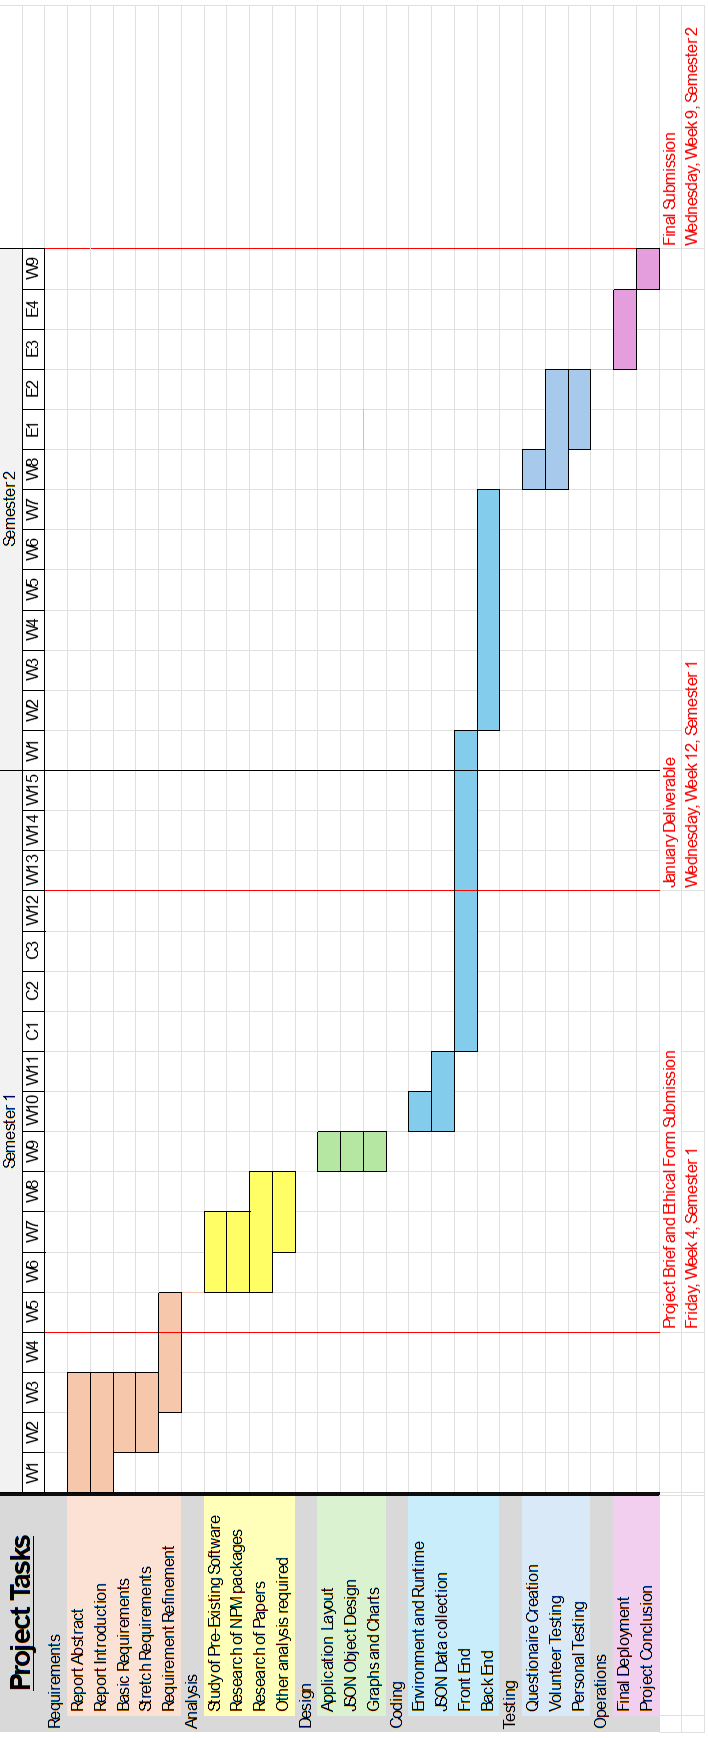
\includegraphics[width=0.4\textwidth, angle=270]{gantt_chart}
        \caption{Gantt Chart}
        \label{fig:gantt_chart}
    \end{figure}
\end{center}
Along with using the Waterfall model, I created a Gantt chart to roughly plan my time for the project. This approach ensures the project is on track against a critical path and establish that I am not spending too much time on one section of the project. I will go into further detail about the Gantt chart in the Methodology section of this report.
\newpage
\chapter{Problem Domain}
For this project, I have elected to use the MoSCoW approach to define the requirements of the project. This specifies the requirements into layers of priority and sets the scope of the project.\\
\begin{itemize}
    \item \textbf{\Large{Must Have (Minimum Viable Product)}}
    \begin{itemize}
        \item The dashboard must show a map of the Earth.
        \item The dashboard must visualise the COVID-19 data and show the number of global cases and deaths per week.
        \item The map will render polygon and country data from a GeoJSON file.
        \item The individual countries must be clickable.
        \begin{itemize}
            \item Clicking a country will update a panel on the right.
            \item The panel will have a time-series graph showing the number of cases and deaths in that country over the time period.
            \item The panel will have another time-series for use in comparison. The user will be able to choose a factor to compare against, such as population, GDP or another country's statistics.
            \item Highlight the secondary country if applicable.
        \end{itemize}
        \item The dashboard must have a timeline slider of the pandemic.
        \begin{itemize}
            \item The user must be able to scrub through the timeline.
            \item There will be a "playback" feature which will automatically scrub through the timeline.
            \item The timeline will show the current week in ISO 8601 format.
        \end{itemize}
        \item Search Bar
        \begin{itemize}
            \item The user must be able to search for a country by name.
            \item The search bar will have a dropdown list of countries.
            \item The dropdown list will be filtered by the user's input.
            \item If an unknown country is entered, the user will be prompted to enter a valid country name.
            \item If a valid country is entered, it will be the same as clicking on the country and the text field will be wiped.
        \end{itemize}
        \item Reactive and responsive design.
        \begin{itemize}
            \item Use of smooth transitions and animations to make the dashboard more visually appealing.
            \item All graphs and functionalities should be connected to the timeline slider and country selected.
        \end{itemize}
    \end{itemize}
    \item \textbf{\Large{Should Have}}
    \begin{itemize}
        \item Zooming in on the map.
        \begin{itemize}
            \item Adding a button to toggle a "zoom" feature on the map.
            \item When clicked, the map will zoom into the selected country.
            \item When clicked again, the map will zoom back out to the world view.
        \end{itemize}
        \item Hotspots on the map.
        \begin{itemize}
            \item This would require analysis of the data to find out where the rate of infection is highest.
        \end{itemize}
    \end{itemize}
    \item \textbf{\Large{Could Have}}
    \begin{itemize}
        \item Analysis of data with other data sources to search for correlations.
        \begin{itemize}
            \item I am currently unsure what data sources I would use for this, but it would be interesting to see if there are any correlations between the spread of the virus and other factors.
            \item Comparing the number of cases or deaths to different countries.
            \item Normalising the data to a GDP per capita basis.
        \end{itemize}
        \item Extensibility to other datasets.
        \begin{itemize}
            \item The code should be generic enough to be used for any pandemic data.
            \item Want to use a generic data format and a script which is able to cast the data into the correct format.
        \end{itemize}
        \item Frame updating to resizing the window.
        \item Removal of spurious and erroneous data at runtime.
    \end{itemize}
    \item \textbf{\Large{Would Have}}
    \begin{itemize}
        \item Predictive modelling and forecasting.
        \begin{itemize}
            \item This is my most ambitious stretch goal. I would like to be able to predict the spread of the virus using the data I have. This would require a lot of work and research into the field of predictive modelling. This would likely be a separate project in itself.
        \end{itemize}
    \end{itemize}
\end{itemize}
\newpage

\chapter{Methodology}
The project incorporates a Waterfall model into my project since it will ensure my code and report as a whole is developed in a structured and ordered fashion.\\
The steps of Waterfall I will be following are:
\begin{enumerate}
    \item \textbf{\large{Requirements}}
    \begin{itemize}
        \item This section involves producing and refining a set of requirements. The requirements are categorized into two groups: Minimum Viable Product requirements and Stretch requirements.
        \item The order of priority for the requirements in this project is defined using the MoSCoW method. This approach ensures that the most critical requirements are addressed first, followed by less essential ones.
        \item All requirements are refined during this stage to maintain a clear and structured project plan.
    \end{itemize}
    \item \textbf{\large{Analysis}}
    \begin{itemize}
        \item This section involves conducting research into the problems identified during the requirement refinement process. Relevant papers and other published sources are investigated to provide insights.
        \item Additionally, an exploration of node packages suitable for graphical data representation is undertaken. This investigation may extend into the design phase.
        \item This section is expected to occupy a significant portion of the report, with potential revisits during the project's progression.
    \end{itemize}
    \item \textbf{\large{Design}}
    \begin{itemize}
        \item The layout and colour scheme of the application would be designed as it would appear in a browser window. Consideration would be given to how different screen sizes might render the application differently, ensuring a responsive design.
        \item Although a database is not being used for this project, JSON will be utilized, and creating a standardized design for objects in JSON would be advantageous.
        \item Decisions would be made regarding the values to be used for graphs and the types of graphs that would best represent the data.
    \end{itemize}
    \item \textbf{\large{Coding}}
    \begin{itemize}
        \item The coding is for a web application with node.js. This will require creation a valid work environment and get the node runtime working on my local machine. The deployment will likely use Docker for this since it is a very easy to work with tool perfect for this application.
        \item The project primarily utilizes JavaScript due to its native compatibility with web development. Additionally, HTML and CSS are employed for loading the D3.js SVGs and aligning elements.
        \item Node.js also comes with node package manager which will also be useful for loading the custom packages I plan on using in this project.
    \end{itemize}
    \item \textbf{\large{Testing and Review}}
    \begin{itemize}
        \item For testing, I will be using a variety of normal, boundary and erroneous tests to check my software for crashes, unexpected results, and vulnerabilities.
        \item Testing will consist of having 3rd-party applicants to test my application. They would have a list of things to do in the application so I can analyse the ease of use.
        \item The testing will abide by all university ethics guidelines and an informed consent form will be signed by the testers after seeing a participant information sheet and relevant risk assessment.
        \item The testers will complete an activity using the tool to extract data and then complete a questionnaire. The questionnaire will ask about the ease of use, the design and the functionality of the application.
        \item I will use the feedback from the testers to improve my application.
    \end{itemize}
    \item \textbf{\large{Operations}}
    \begin{itemize}
        \item I want to deploy my application to a docker container and eventually a server.
        \item Node.js applications are commonly deployed onto servers and having a production repository would be a good standard for myself. Pushing to a server from a local git repository is a highly transferable skill which is widely used.
    \end{itemize}
\end{enumerate}

\newpage
\chapter{Literature Review}
\section{Existing Solutions}
\subsection{COVID-19 Dashboard}
A common tool for data visualisation is a software called PowerBI, a Microsoft product which allows for the creation of dashboards. 
The dashboard in the figure shows a real-time representation of the COVID-19 pandemic.
\begin{center}
    \begin{figure}[h]
        \centering
        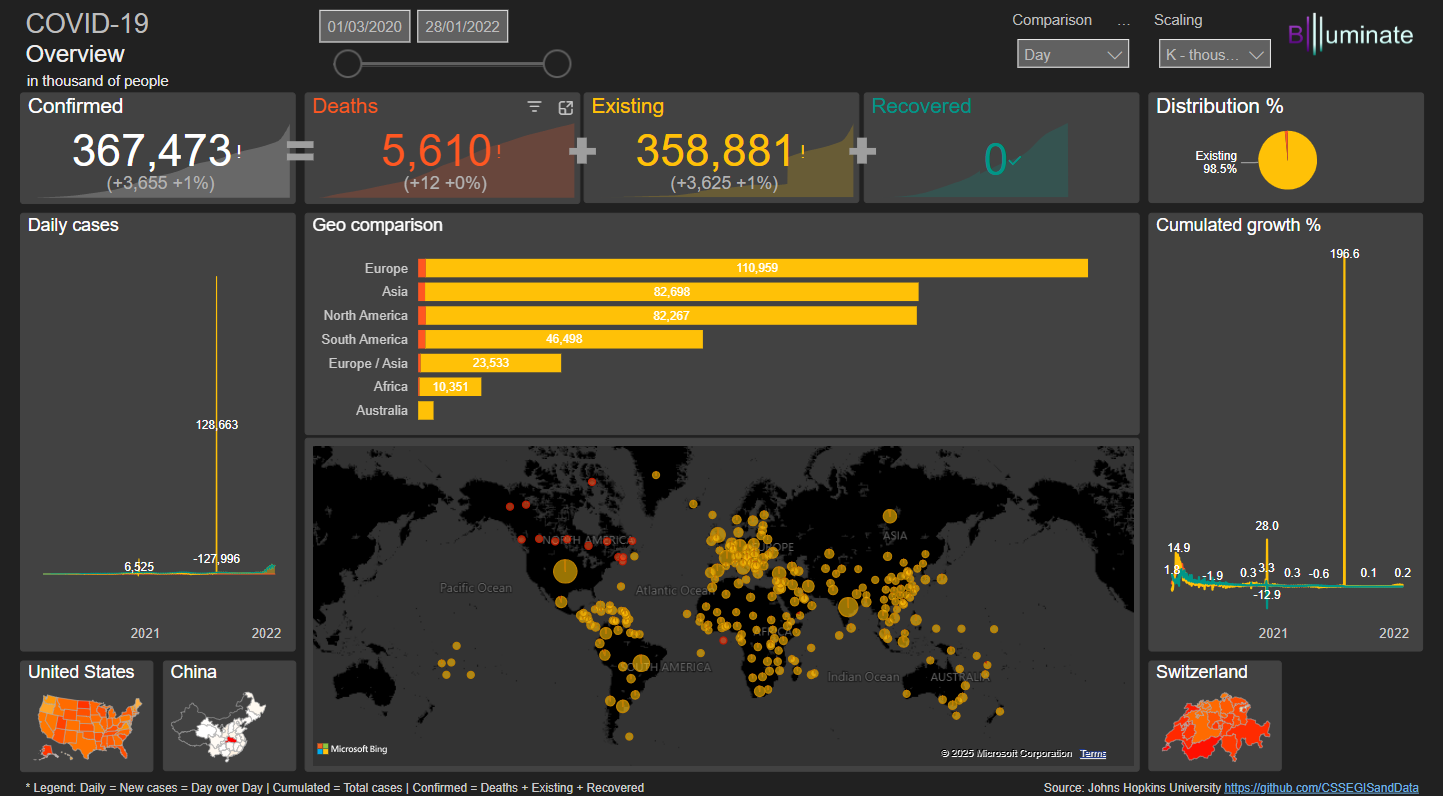
\includegraphics[width=0.95\textwidth]{PowerBI Example.png}
        \caption{COVID-19 Dashboard Example \cite{Badr2023}}
        \label{fig:covid19_dashboard}
    \end{figure}
\end{center}
This dashboard has a broad spectrum of information even at first glance. The map uses bubbles to denote hotspots of activity for the virus. The bubbles are sized by the number of cases in that country. The bubbles can also be clicked for more detailed information on that country. \\
The user is also able to alter the time frame of the data, and the data is updated in real time.\\
There is a lot here which I would like to incorporate into my own project. The map is a good way to visualise the data and the bubbles are a good way to show the number of cases in each country. I also like the big bold text which summarises the data which is easy to read.\\
\newpage
\subsection{Plague Inc.}
Plague Inc. is a game published in 2012 by Ndemic Creations. It gives the user the ability to create and spread a virus across the world. The game was initially released on mobile devices and has since been released on PC and console. \cite{plagueinc}\\
Mobiles games require accessible and easy to use interfaces, which is why Plague Inc. is a good example of a visual pandemic simulation. The game is simple to use and has a lot of information on the screen at once.
\begin{center}
    \begin{figure}[h]
        \centering
        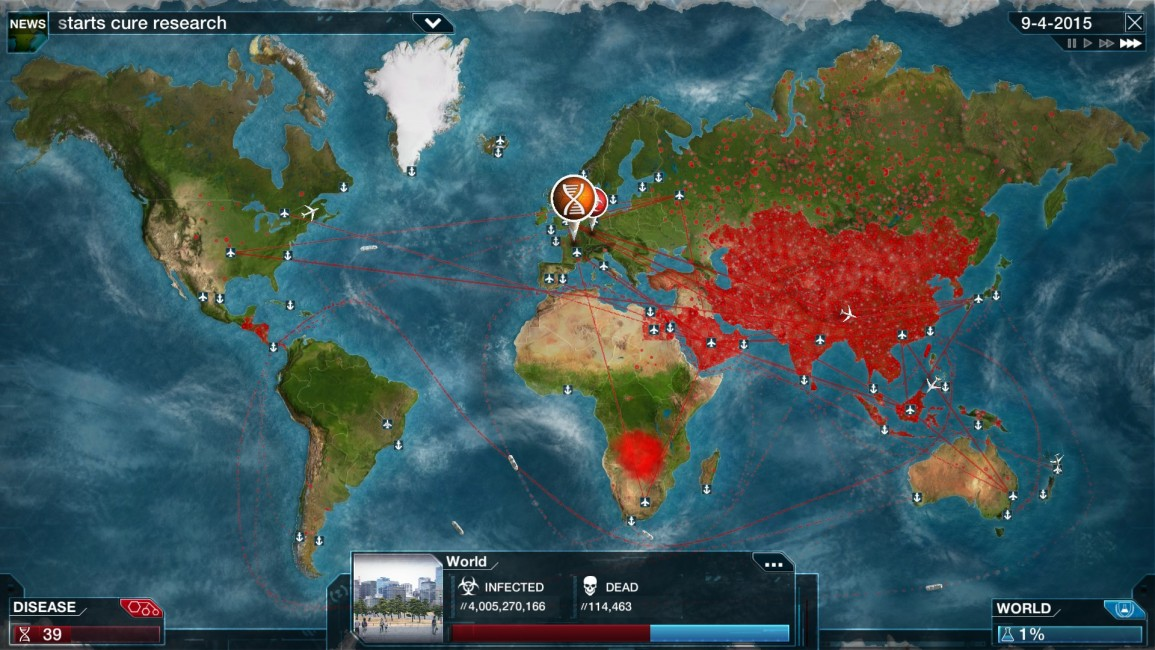
\includegraphics[width=0.95\textwidth]{Plague Inc Example.jpeg}
        \caption{Plague Inc. Dashboard Example}
        \label{fig:plagueinc_dashboard}
    \end{figure}
\end{center}
Despite many systems being dramatised for the sake of gameplay, the game offers many features which could be useful for a real-world pandemic simulation. \\
The game uses a world map which gradually changes colour as the virus spreads, this is from many red dots appearing on the map. The user also has access to individual breakdowns of each country and can see the number of cases and deaths in each country.\\ 
The game also has a transmission system which changes from country to country. 
\\ \\
There is certain information provided in these examples that I will not be able to provide in my project. For example, the COVID-19 dashboard has real-time data, which I will not be able to provide. The Plague Inc. game has a transmission system which shows the spread country to country, which I will not be able to provide.\\
\newpage
\section{Data Sources}
The data for this project will be sourced from the European Centre for Disease Prevention and Control (ECDC) \cite{ecdc}. The data is historic and only has data from the 1st week of 2020 to the 23rd week of 2022. The data is in a JSON format and includes the number of cases and deaths per week for each country. The format of the data is as follows:

\begin{minipage}{0.45\textwidth}
\begin{lstlisting}[caption={Cases JSON Example}]
{
    "country": "Afghanistan",
    "country_code": "AFG",
    "continent": "Asia",
    "population": 38928341,
    "indicator": "cases",
    "weekly_count": 1368,
    "year_week": "2020-47",
    "rate_14_day": 6.5043,
    "cumulative_count": 44771,
    "source": "Epidemic intelligence national data"
}
\end{lstlisting}
\end{minipage}
\hfill
\begin{minipage}{0.45\textwidth}
\begin{lstlisting}[caption={Deaths JSON Example}]
{
    "country": "Afghanistan",
    "country_code": "AFG",
    "continent": "Asia",
    "population": 38928341,
    "indicator": "deaths",
    "weekly_count": 69,
    "year_week": "2020-47",
    "rate_14_day": 3.3395,
    "cumulative_count": 1695,
    "source": "Epidemic intelligence national data"
}
\end{lstlisting}
\end{minipage}

This is the format that the ECDC provide, but I will be amending it slightly to make it easier to work with. I will be combining the cases and deaths into one object and adding a date field. This will make it easier to work with the data in the front end.\\

It also needs to correspond with the GeoJSON data I will be using to render the map. \\

It is worth noting that I don't want this code to be limited to just COVID-19 data. I want to be able to use this code for any pandemic data. This is why I am making the data more generic and easier to work with.
\newpage
\section{Compartmental Models}
\subsection{SIR Model}
Compartmental models are a type of mathematical model used to represent the different populations in a system. The most common compartmental system in epidemiology is the SIR model \cite{beckley2013modeling}.\\
The SIR model is a simple model which divides the population into three compartments: Susceptible, Infected and Recovered. The model is represented by the following differential equations:
\begin{align}
\frac{dS}{dt} &= -\alpha SI \label{sir_model_dS} \\
\frac{dI}{dt} &= \alpha SI - \beta I \label{sir_model_dI} \\
\frac{dR}{dt} &= \beta I \label{sir_model_dR}
\end{align}
Where:
\begin{itemize}
    \item S is the number of susceptible individuals.
    \item I is the number of infected individuals.
    \item R is the number of recovered individuals.
    \item $\alpha$ is the rate of infection.
    \item $\beta$ is the rate of recovery.
\end{itemize}
To explain this model, it's important to understand proportional reasoning. In the first equation, \ref{sir_model_dS}, the rate of change of the susceptible population is proportional to the complement of the product of the susceptible and infected populations.\\
A way to think of why that is true is because the more infected people there are, the more likely it is for a susceptible person to become infected.\\
This model is a good starting point for understanding the spread of a virus, but it has some limitations. In this model, once you have recovered, you are no longer able to be infected. Another issue is that the model assumes the disease is non-fatal.

\begin{center}
    \begin{figure}[h]
        \centering
        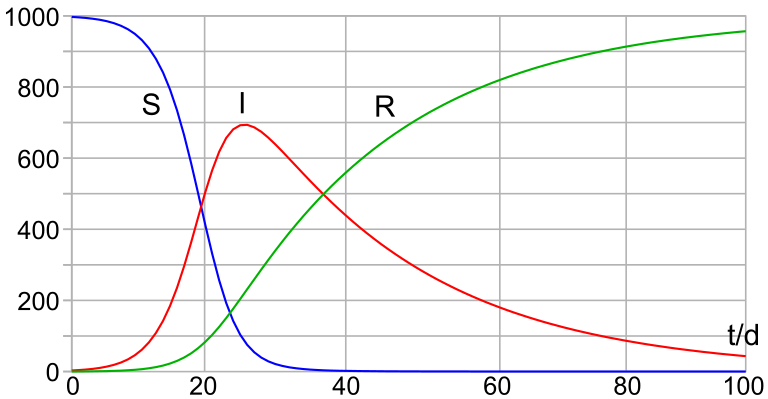
\includegraphics[width=0.8\textwidth]{SIR-Model.png}
        \caption{Diagram of SIR Model with start values S=997, I=3, R=0, $\alpha$=0.0004, $\beta$=0.04. \cite{sirmodel}}
        \label{fig:sir_model}
    \end{figure}
\end{center}

\subsection{Solution to the SIR Model}
The SIR model can be solved using numerical methods. The most common method is the Euler method. The Euler method is a simple method for solving ordinary differential equations. It is not the most accurate method, but it is easy to implement. The Euler method is represented by the following equations:
\begin{align}
S_{n+1} &= S_n - \alpha S_n I_n \Delta t \label{sir_euler_S} \\
I_{n+1} &= I_n + \alpha S_n I_n \Delta t - \beta I_n \Delta t \label{sir_euler_I} \\
R_{n+1} &= R_n + \beta I_n \Delta t \label{sir_euler_R}
\end{align}
Where:
\begin{itemize}
    \item $S_n$ is the number of susceptible individuals at time $n$.
    \item $I_n$ is the number of infected individuals at time $n$.
    \item $R_n$ is the number of recovered individuals at time $n$.
    \item $\Delta t$ is the time step.
\end{itemize}
If we look at the phase space of the SIR model, we can see that the model has a fixed point at the origin. This means that the model will always return to the origin. This is not the case in real life, as the disease will eventually die out. This is because the model does not take into account the finite population size.
\subsection{Improvements to the SIR Model}
The SIR model can be improved by adding more compartments to the model. However, this makes the model more complex and harder to solve.
\subsubsection{SEIR Model}
This model adds an exposed compartment to the SIR model. For individuals who have been infected but are not yet infectious. The model is represented by the following differential equations:
\begin{align}
\frac{dS}{dt} &= \mu N - \mu S - \frac{\beta IS}{N} \label{seir_model_dS} \\
\frac{dE}{dt} &= \frac{\beta IS}{N} - (\mu + a)E \label{seir_model_dE} \\
\frac{dI}{dt} &= aE - (\mu + \gamma)I \label{seir_model_dI} \\
\frac{dR}{dt} &= \gamma I - \mu R \label{seir_model_dR}
\end{align}
The SEIR model is better for simulations than the SIR model since it takes into account the incubation period of the disease. This is important as it is possible for a person to be infected but not yet infectious.\\

It is beyond the scope of this project to go into detail about the SEIR model, but it is worth noting that the model is more complex and requires more data to solve. The model is also more accurate than the SIR model.
\newpage
\section{Statistical Analysis}
Statistical analysis is a key part of this project. I will be using statistical analysis to find correlations between the data and other factors. I will be comparing the cumulative cases and deaths of two countries to see if there are any correlations between the two.\\

I also want to make a statistic comparing the number of cases to the gdp per capita of the country to see if there is an inverse correlation between the two. This would be interesting to see richer countries were able to contain the virus better than poorer countries.
\begin{align}
\text{Infections} &\propto \frac{1}{\text{GDP Per Capita}}
\end{align}

If this is the case, I would like to calculate the constant of proportionality. This would be a good indicator of how much money a country needs to spend to contain the virus. \\

I would also like to compare number of cases to other statistics I have available to me in my GeoJSON file. This includes:
\begin{itemize}
    \item Population
    \item Sovereign status
    \item Type of economy
    \item etc
\end{itemize}

\newpage
\chapter{Design Review}
\section{Wire-framing}
I need to work within the constraints of node.js and D3.js for my designs. Below is a wire-frame of the dashboard I plan on creating.
\begin{center}
    \begin{figure}[h]
        \centering
        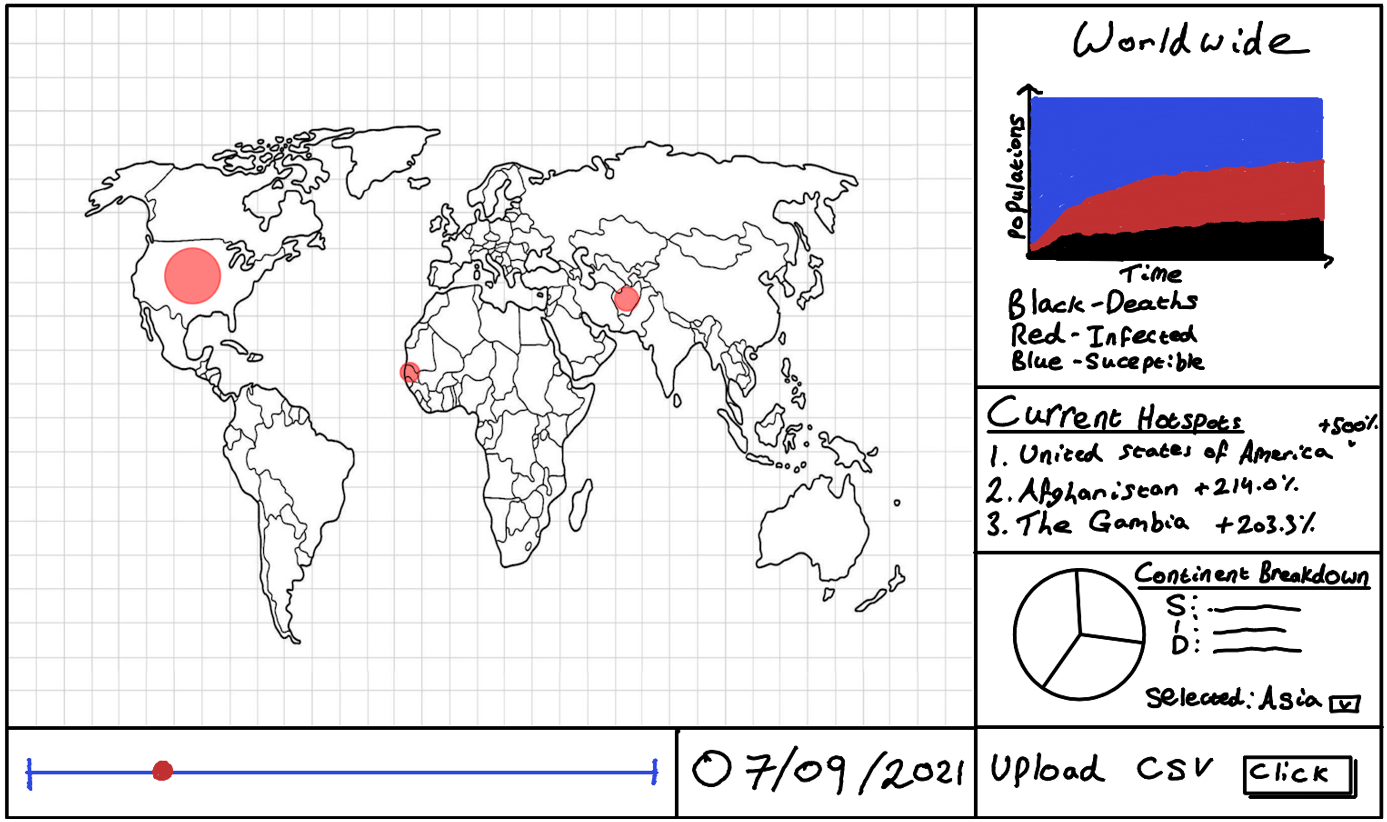
\includegraphics[width=0.95\textwidth]{Images/Home_Wireframe.png}
        \caption{Wireframe of Dashboard}
        \label{fig:wireframe_world}
    \end{figure}
\end{center}
Specific features of the dashboard include:
\begin{itemize}
    \item A map of the Earth.
    \item An interactive timeline of the pandemic.
    \item A area chart showing the number of cases, deaths and population susceptible.
    \item Listed hotspots and the percentage change within the countries.
    \item Hotspots on the map.
    \item A pie chart for susceptible, infected and dead populations within continents.
    \item A button to load different data files.
    \item The current date in the data.
\end{itemize}
When clicking on a country, the canvas will zoom onto the country, giving more specific information on how the pandemic is affecting that country. A button will also be available to return to the world map.
\begin{center}
    \begin{figure}[h]
        \centering
        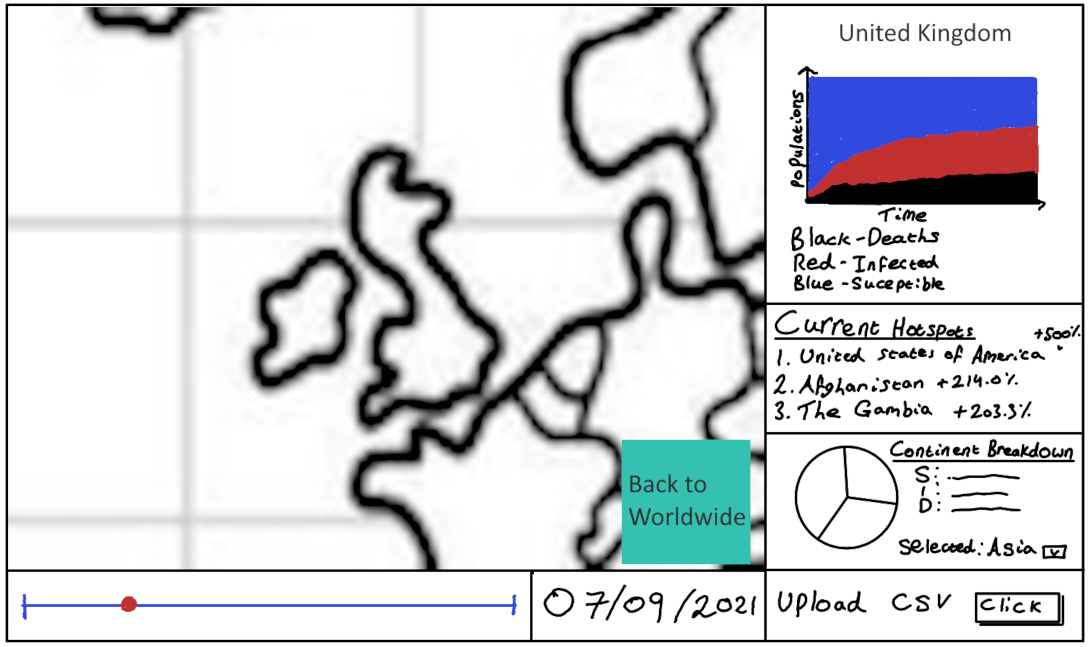
\includegraphics[width=0.95\textwidth]{Images/Country_Wireframe.png}
        \caption{Wireframe of Country Page}
        \label{fig:wireframe_country}
    \end{figure}
\end{center}
A perk of using SVG to render the map is that when zooming, no resolution is lost. This is because SVG is a vector format, meaning that the image is made up of lines and shapes rather than pixels. This means that the image can be scaled up and down without losing quality.
\section{D3.js}
D3.js is a JavaScript library for producing dynamic, interactive data visualisations in web browsers. It makes use of the widely supported SVG format to render graphics. D3.js is a powerful tool for creating visualisations and is widely used in industry.\\

D3.js is a good choice for this project as it natively supports GeoJSON data which is the format I will be using for the map. The polygon data is open source. \cite{geojsonvectormaps}\\

This is exclusively used on a web browser, so I will be using node.js to serve the data to the front end.\\

D3.js also has many built-in functions for creating different types of graphs and charts and interacting with them. As an example, D3.js has a built-in function for calculating the bounding box of a country polygon. I will be using this function to calculate where to zoom in on the map. Here's a JavaScript snippet of how I will be using this function:

\begin{lstlisting}[language=JavaScript]
// Creates a 2d array of the bounding box of the country
const bounds = path.bounds(d);
const dx = bounds[1][0] - bounds[0][0];
const dy = bounds[1][1] - bounds[0][1];
const x = (bounds[0][0] + bounds[1][0]) / 2;
const y = (bounds[0][1] + bounds[1][1]) / 2;

// Calculate the scale of the zoom
const scale = Math.max(1, Math.min(8, 0.9 / Math.max(dx / width, dy / height)));
const translate = [width / 2 - scale * x, height / 2 - scale * y];

// Smoothly transition to the new zoom level
svg.transition()
    .duration(750)
    .call(
        zoom.transform,
        d3.zoomIdentity.translate(translate[0], translate[1]).scale(scale)
    );
\end{lstlisting}

The GeoJSON data has much more information than the COVID-19 data. It includes geometry of the country, information regarding the countries economy, sovereign status, GDP, all in multiple languages. I will be cleaning the data to only include relevant information for this project: country name in English, country code (to link the data with the Covid-19 JSON file) and geometry information. 

\section{Chloropleth Maps}
For this project, I referred to a book on data visualisation by Andy Kirk \cite{andy2019kirk}. The book is a good introduction to maps with data visualisation as well as the use of colour in maps making it a good resource. \\

\begin{wrapfigure}{l}{0.4\textwidth}
    \begin{center}
      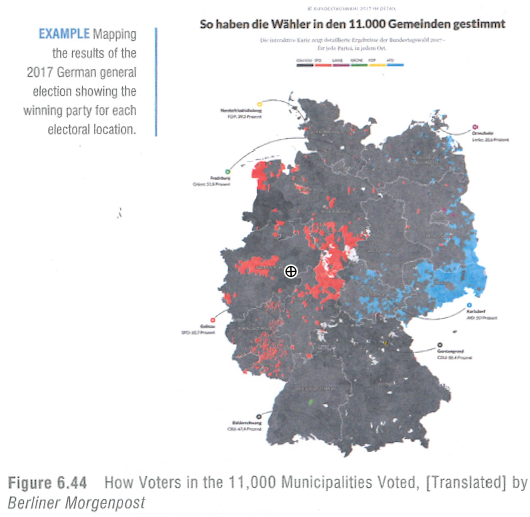
\includegraphics[width=0.38\textwidth]{chloropleth-example.png}
    \end{center}
    \caption{Example Chloropleth Map from Andy Kirk's Book \cite{andy2019kirk}}
  \end{wrapfigure}

Choropleth maps are a type of map which uses colour to represent data. The map is divided into regions and each region is coloured based on the data. This is a good way to visualise data as it allows for easy comparison between regions.\\

The figure on the left is colouring the regions based on different voter populations in Germany. This differs to how I will be using chloropleth. My legend will be a logarithmic scale from white to red to signify the number of cases in that region. The darker the red, the more cases there are in that region.\\

The reason I am choosing a logarithmic scale is due to the disparity of the numbers, especially in the early days of the pandemic. The logarithmic scale allows for a better visualisation of the data as it allows for a wider range of values to be represented. It is commonly the used scale for pandemic data.

\newpage
\chapter{Technical Solution}
\section{Node.js}
Before I start working on any code, I need to set up my development environment. As I discussed in my design section, I will be using node.js to serve data in front end and D3.js to render the data.\\

This is my first time using node.js and web development in general, so I spent a lot of time researching how to set up a node.js server. The first step I took was to install node.js on my local machine. I intend on deploying the application to a server hosted by the university using a Docker container, but I will be developing the application on my local machine.\\

I used the express.js framework to create a simple server with a router to serve the data. I have a diagram of the structure of my router schema below.

\begin{center}
    \begin{figure}[h]
        \centering
        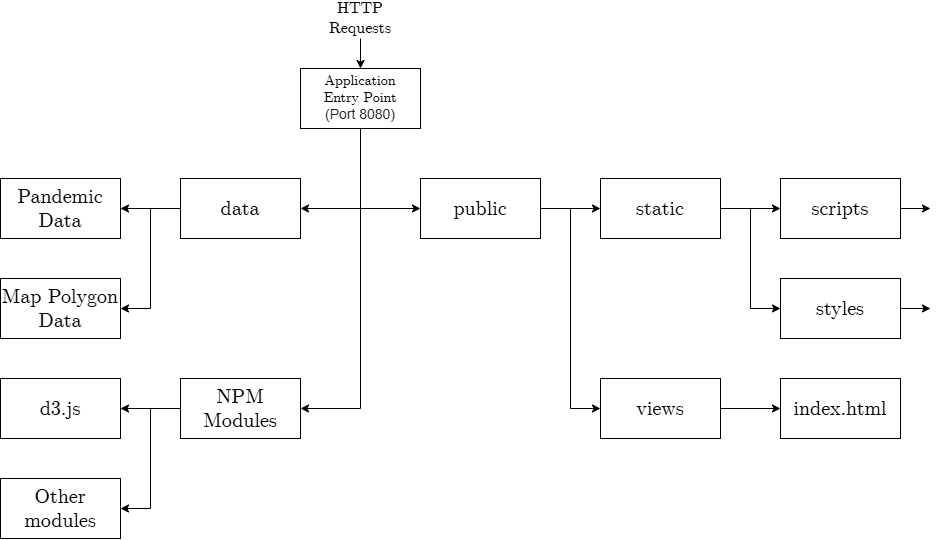
\includegraphics[width=0.95\textwidth]{Images/router_scheme.drawio.png}
        \caption{Data Routing Structure}
        \label{fig:nodejs_structure}
    \end{figure}
\end{center}

\section{Asynchronous Data Fetching}
When dealing with data in JavaScript, and web programming as a whole, you must deal with asynchronous data fetching. This is because the data is not available immediately and the program must wait for the data to be fetched before it can be used. In my project, I used the fetch API to fetch the data. The word "server" in this context is a bit misleading, as the data is not being served from a server, but rather a local file. In node.js, the lines between server and client are blurred, as the server is also the client.\\

The fetch API is a promise-based API which returns a promise object. This means that the data is not available immediately and the program must wait for the data to be fetched. If the promise is resolved, it will contain the okay response of "200", and the data requested. If the promise is rejected, for example if the file is not found, it will contain the error message with an error code.\\ 

Because of the chance of the promise being rejected, I used error validation and a catch statement to handle the error. This is a good practice when dealing with asynchronous data fetching, as it allows for better error handling and debugging. Here is an example of how I used the fetch API to fetch the data:
\begin{center}
    \begin{lstlisting}[language=JavaScript]
    fetch('https://api.example.com/data')
    .then(response => {
        if (!response.ok) throw new
                Error('Network response was not ok'); // #404
        return response.json();
    })
    .then(data => {
        console.log('Data received:', data); // #200
        // Process the data here
    })
    .catch(error => {
        console.error('Fetch error:', error);
    });
    \end{lstlisting}
\end{center}

On the next page is a sequence diagram of the data fetching process. The diagram shows the flow of data from the server to the client and how the data is fetched asynchronously.\\

\newpage
\begin{center}
    \begin{figure}[h]
        \centering
        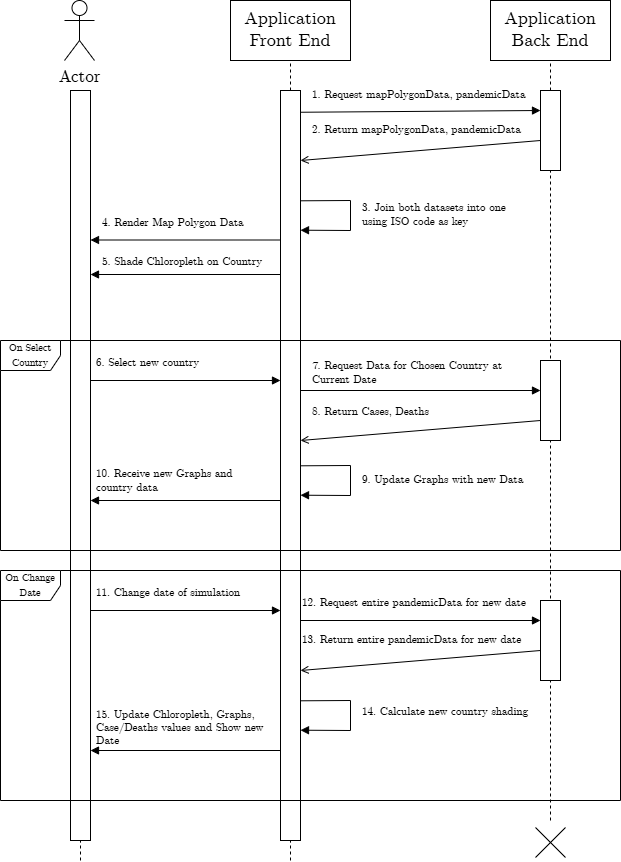
\includegraphics[width=0.8\textwidth]{Images/sequence_diagram.drawio.png}
        \caption{UML Sequence Diagram for Asynchronous Data Fetching}
        \label{fig:sequence_diagram}
    \end{figure}
\end{center}
\newpage

\newpage
\section{Cleaning the Data}
Before I start working on the front end, I need to clean the data. The data from the ECDC is in a JSON format, but it is not in a format that is easy to work with. I need to combine the cases and deaths into one object and add a date field. This will make it easier to work with the data in the front end.\\

I will be using Python to clean the data, since doing this is a one-time task and Python is a good language for data manipulation. I will be using the json library to read the JSON file and the defaultdict package to manipulate the data into a standardised form. I will then write the cleaned data to a new JSON file.\\

I restructured the data to look like this:
\begin{center}
    \begin{lstlisting}
    {
        "AFG": {
            "properties": {
                "country": "Afghanistan",
                "country_code": "AFG",
                "continent": "Asia",
                "population": 38928341,
                "source": "Epidemic intelligence national data"
            },
            "data": {
                "2020-01": {
                    "cases": 0,
                    "deaths": 0,
                    "cumulative_cases": 0,
                    "cumulative_deaths": 0,
                    "rate_14_day_cases": 0.0,
                    "rate_14_day_deaths": 0.0
                },
                [...]
            }
        },
        [...]
    }
    \end{lstlisting}
\end{center}
The python code I used can be found in the appendix.

\section{Country Selection}
For this project, I need to decide on what list of countries to use. The GeoJSON file I will be using has a selection of countries, but a definitive list of countries doesn't exist.\\

There are multiple countries that are in dispute due to political or territorial reasons. For example, Taiwan is not recognised as a country by the United Nations due to China needing to agree, but it is a country in its own right. I will be including Taiwan in my list of countries.\\

Another consideration are countries which aren't included in the $\mathbf{ISO}$ $\mathbf{3166-1}$ $\mathbf{Alpha-3}$ country code set which is what both the ECDC and GeoJSON file use. An example is Somaliland which is a self-declared state but is not recognised by the United Nations or the ISO-3166-1 country code, but the dataset does contain data so we will extend the country code set to include this.\\

There are more examples like this, but I will not mention every single one. I will be using the ISO-3166-1 country code set as a base, but I will be extending it to include countries which are not recognised by the United Nations for which I have data on.\\
\newpage
Initially, I wanted to use UNIX timestamps to store the date, but I have since changed my mind. This is because of of how the HTML slider tag works. The slider expects consistent step values, and UNIX timestamps are not consistent due to daylight savings time.\\

To combat this, I am storing data in the string form of "YYYY-ww" where YYYY is the year and ww is the week number. This is a consistent format and will work with the HTML slider tag. I will have a function to convert the string to a date object when I need to use it. It is also ISO 8601 compliant, which is a common standard for this type of data.

\section{Frontend}
\subsection{User Interface and Experience}
Below is my dashboard created using D3.js and HTML.
\begin{center}
    \begin{figure}[h]
        \centering
        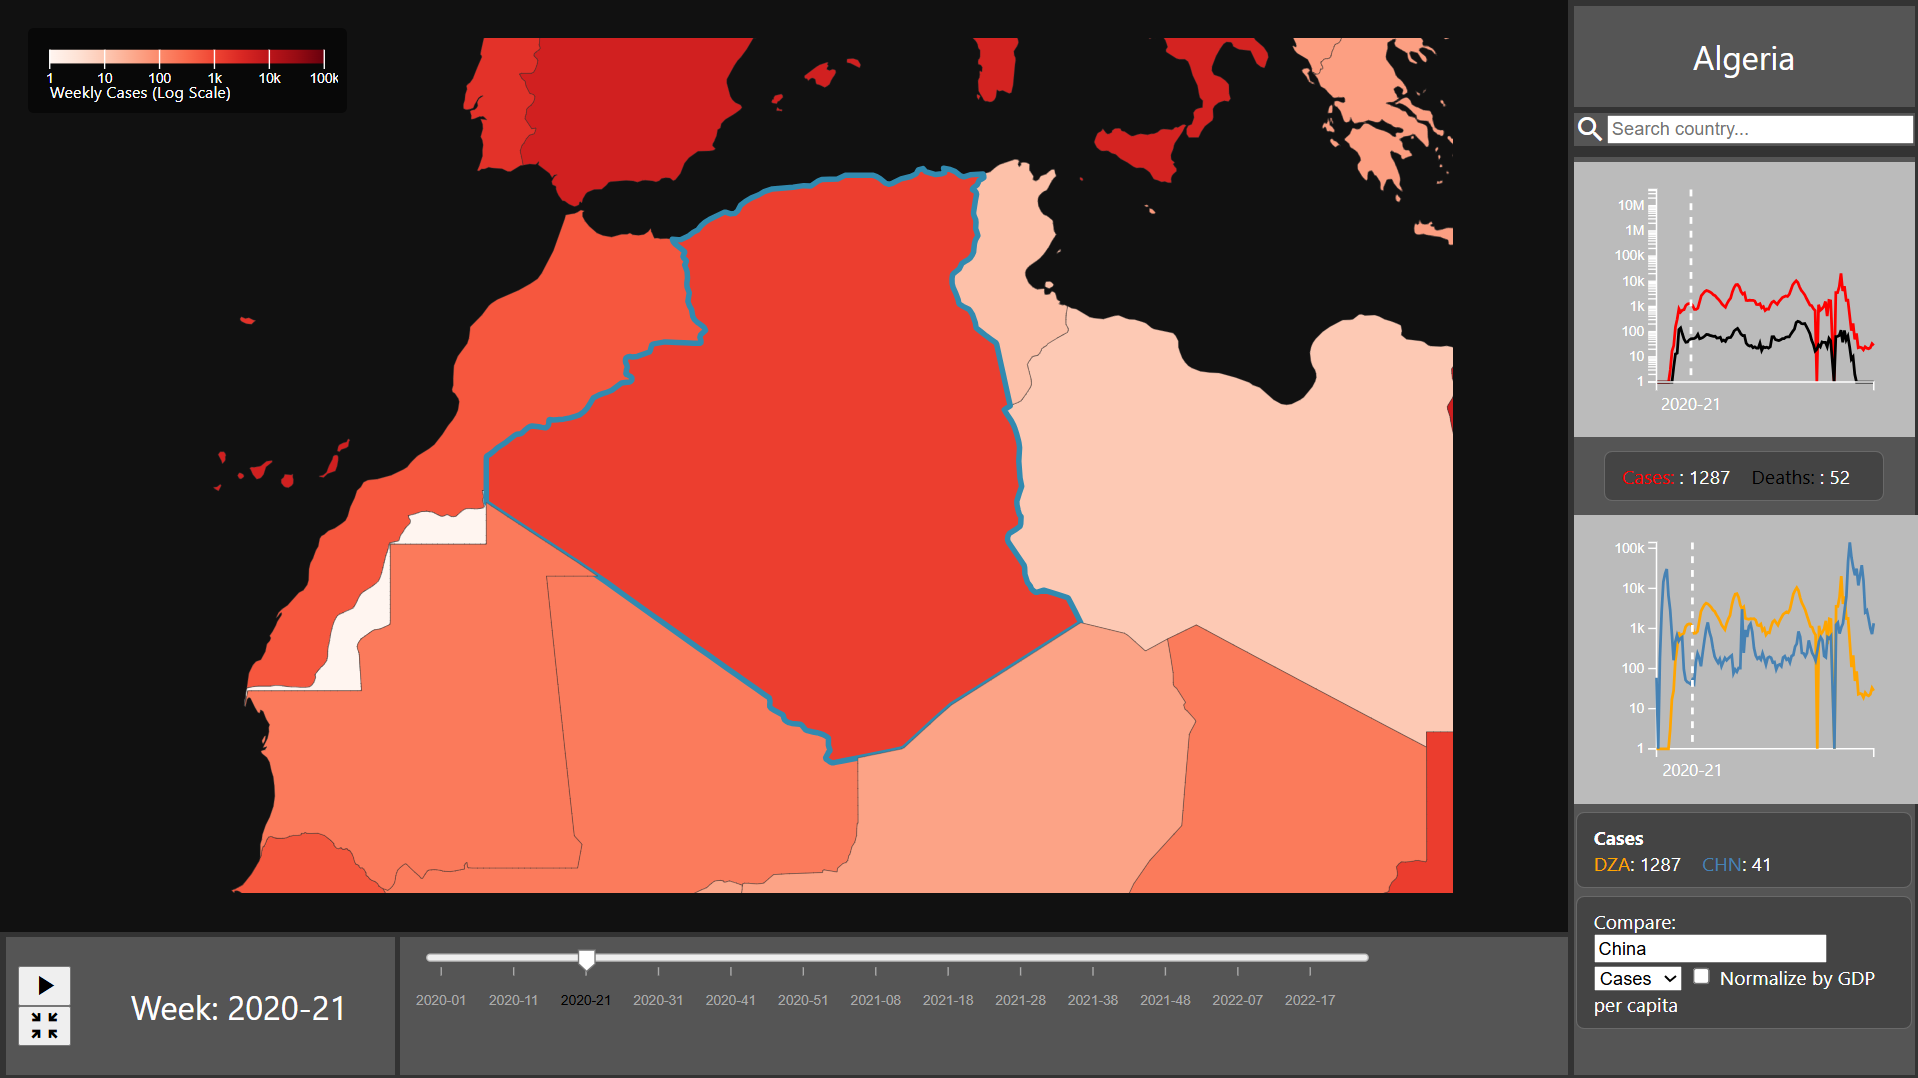
\includegraphics[width=0.95\textwidth]{Images/dashboard.png}
        \caption{Dashboard}
        \label{fig:dashboard}
    \end{figure}
\end{center}
I will go into more detail about the features of the dashboard in the coming sections.
\subsection{World Map}
The world map in this project was a success in planning. I used the D3.js library to render the map and it worked well. The map is interactive and allows the user to zoom in on countries.

I was able to take advantage of features in D3.js like transition and zoom for a smoother feel to the map. The chloropleth map is a good way to represent the data and allows the user to see the hotspots of the virus.

I used the GeoJSON polygon data to render the map. This had many beneficial side effects, like: Choice of projection, the multipolygon feature of GeoJSON, rendering the data in SVG format, and the ability to use D3.js features like transitions and zoom.

\subsection{Info Panel}
The info panel is a div which is activated when a country is clicked. The div contains information about the country and the data. The information is displayed in a table format. The table contains the following information:
\subsubsection{Country Graph}
I initially planned to use a stacked area chart for this project, but I have since changed my mind. The reason is that the stacked area chart does not properly represent the data when used with a logarithmic scale. The populations of the susceptible and the cases/deaths are very disproportionate so a linear scale would not work. Instead, I will be using a logarithmic scale for the y-axis and have multiple lines on the same graph. This will allow me to show the data in a more meaningful way.
\subsubsection{Comparison Graph}
The comparison graph is a simple line chart with a logarithmic scale. The x-axis is the date and the y-axis is the number of cases/deaths. The country is able to be changed as well as the type of data. The options of data I chose to include are:
\begin{itemize}
    \item Cases
    \item Deaths
    \item Cases per GDP per capita
    \item Deaths per GDP per capita
\end{itemize}
I intended on having more options, however I was unsure that a line graph would be the best way to represent the data with a binary part like Sovereign status.
\subsection{Search Bar}
The search bar is a simple input field which is designed to behave the same as just clicking a country. The user can type in the name of the country, and the field will show a list of countries which match the input. The user can then click on the country and the map will zoom in on the country. This is a good way to allow the user to find a country quickly without having to scroll through the map.

\subsection{Zoom}
I used a "zoom mode" in my application. It has functionality when a country is selected and sets the bounding box of the country to the view. This code also allows the user to freely zoom in and out of the map, and pan around the map. This is a d3.js feature which is used extensively.

\subsection{Live Playback}
The application has a live playback feature which allows the user to see how the data progresses over time. The user can click on the play button and the application will automatically update the data every week. When the button is clicked, it becomes a toggle button which allows the user to pause the playback. The playback automatically stops when the end of the data is reached.

\subsection{Week Slider}
The slider is a d3.js slider which allows the user to select a week. It required some logic to cast the position on the slider to a week. The slider is a good way to to allow the user to select a week without having to type in the date.

\section{Backend}
For the data in my application, I am using the file "interface.js" to load the data from the JSON file. This file is an async module which exports a function to load the data. The function can fetch all data or data specified in the parameters. The function will return a promise which resolves to the data. This is a simple way to load data from a file and is a common pattern in JavaScript.

\section{Deployment}
In this project, I used Docker to deploy my application. Docker is a containerisation platform which allows you to package your application and all its dependencies into a single container. The only prerequisite is that the host machine has the Docker engine installed. This is a good way to deploy applications as it allows for easy deployment and scaling.\\

I only used Docker in the production environment, as I was developing the application on my local machine. In the README file of my project, I have included instructions on how to run the application in both the node.js runtime and the Docker container.\\

I decided against using the Docker image to run the data cleaning script for debugging purposes. But Docker would be a good solution because of the dockerfile's capability for "layers". If the data has been cleaned already, the dockerfile will not need to run the data cleaning script again. \\

In my Dockerfile, I used the node.js runtime as the base image, and then copied the files into the container. I then installed the dependencies using npm and exposed the port 8080. You can see the Dockerfile below:

\begin{figure}[h]
    \centering
    \begin{lstlisting}[language=Docker]
        FROM node:20

        WORKDIR /app

        COPY package*.json ./
        RUN npm install

        COPY . .

        EXPOSE 8080

        CMD ["npm", "start"]
    \end{lstlisting}
    \caption{Dockerfile for the Application}
    \label{fig:dockerfile}
\end{figure}
\begin{center}
    \begin{figure}[h]
        \centering
        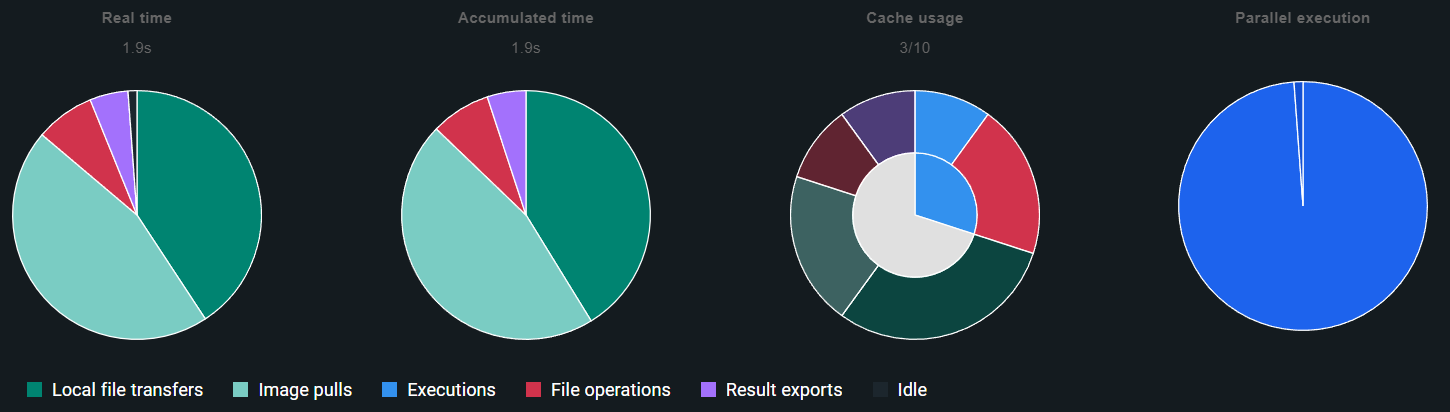
\includegraphics[width=0.95\textwidth]{Images/docker-build.png}
        \caption{Building the Docker Image}
        \label{fig:docker-build}
    \end{figure}
\end{center}

\chapter{User Analysis}
For this section, I conducted user testing on my application. I lead the testers through an activity where they had to use the application and extract information from it. I then asked them what they thought of the application and if they had any suggestions for improvement.\\

I followed the LEON ethics guidelines for this project, producing an informed consent form, participant information sheet, risk assessment and an approved questionnaire. I also made sure to anonymise the data and not use any personal information.
\section{User Testing and Review}
The first set of questions was in regards to the UI and UX of the application and how easy it was to use. These were the questions asked:\\ \\
\textbf{Question 1: }By clicking the country, select Egypt\\
\textbf{Question 2: }Using the zoom button, zoom into Egypt.\\

\noindent
\begin{minipage}[t]{0.45\textwidth}
    \centering
    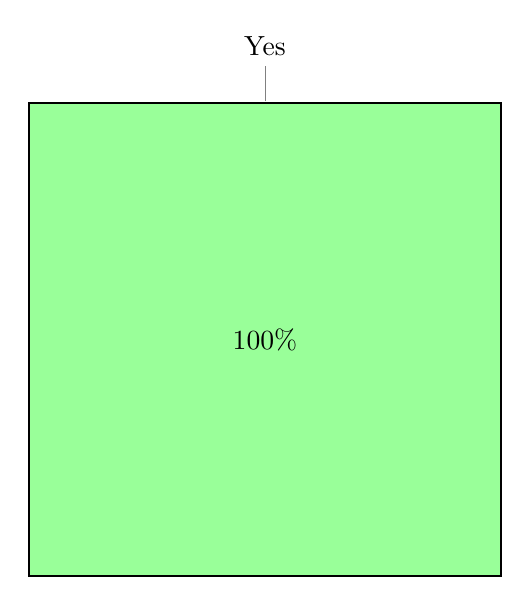
\begin{tikzpicture}[scale=1]
        \pie[square, text=pin, color={green!40, red!30, red!40}]{100/Yes}
    \end{tikzpicture}
    \captionof{figure}{Question 1 Results}
\end{minipage}
\hfill
\begin{minipage}[t]{0.45\textwidth}
    \centering
    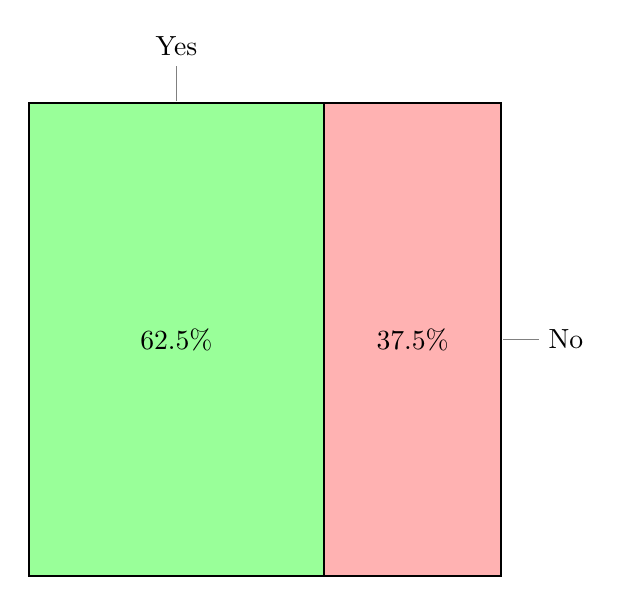
\begin{tikzpicture}[scale=1]
        \pie[square, text=pin, color={green!40, red!30, red!40}]{62.5/Yes, 37.5/No}
    \end{tikzpicture}
    \captionof{figure}{Question 2 Results}
\end{minipage}
\newline
\\There was no issue with the first question, all users were able to select a country and see the corresponding data. However, the second question caused some issues. The main issue with the zoom feature was that the button to activate the zoom mode was not clear. The users were confused about how to activate the zoom mode and some of them did not know that they could click on the map to zoom in.\\

The next set of questions was in regards to getting data from the application. I had 4 questions in this section: \\ \\
\textbf{Question 3: }How many cases of Covid-19 was recorded in the 20th week of 2020 in Egypt? \\
\textbf{Question 4: }Using the comparison graph, did Egypt or South Africa have more deaths on the 45th week of 2020?\\
\textbf{Question 5: }On what week did Sweden have it's peak case count?\\
\textbf{Question 6: }Compare the cases per GDP between United Kingdom and Germany on the week 2021-48, which country had more cases per GDP? \\ \\
The results of the questions are below:\\
\noindent
\begin{minipage}[t]{0.45\textwidth}
    \centering
    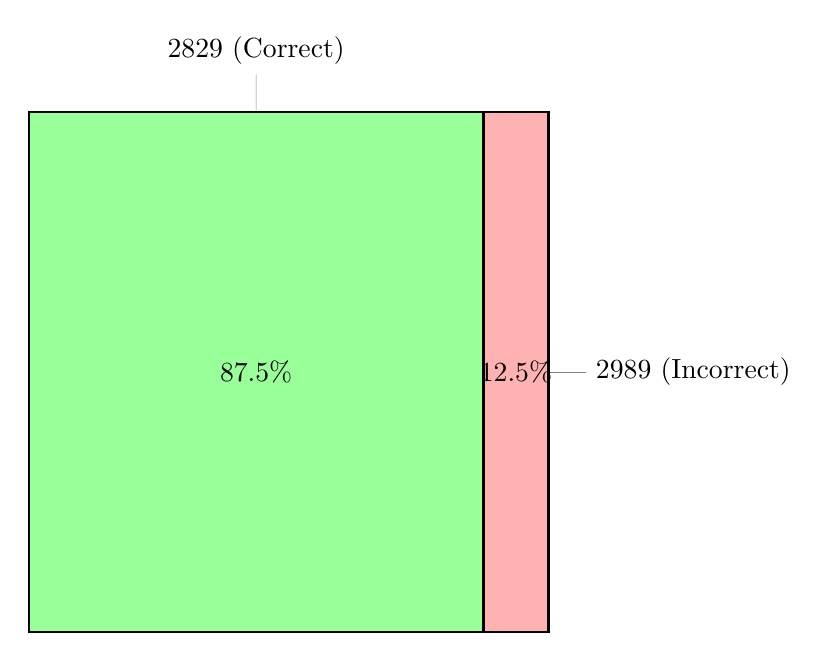
\begin{tikzpicture}[scale=1.1]
        \pie[square, text=pin, color={green!40, red!30, red!40}]{87.5/2829 (Correct), 12.5/2989 (Incorrect)}
    \end{tikzpicture}
    \captionof{figure}{Question 3 Results}
\end{minipage}
\hfill
\begin{minipage}[t]{0.35\textwidth}
    \centering
    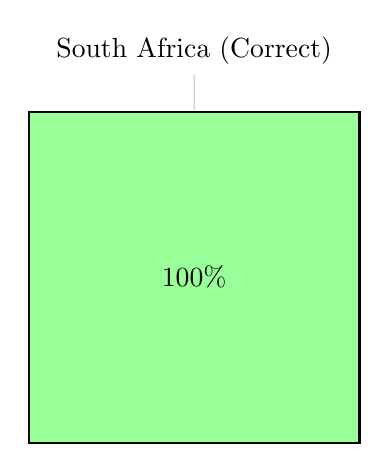
\begin{tikzpicture}[scale=0.7]
        \pie[square, text=pin, color={green!40, red!30, red!40}]{100/South Africa (Correct)}
    \end{tikzpicture}
    \captionof{figure}{Question 4 Results}
\end{minipage}
\vspace{1cm}
\begin{minipage}[t]{0.45\textwidth}
    \centering
    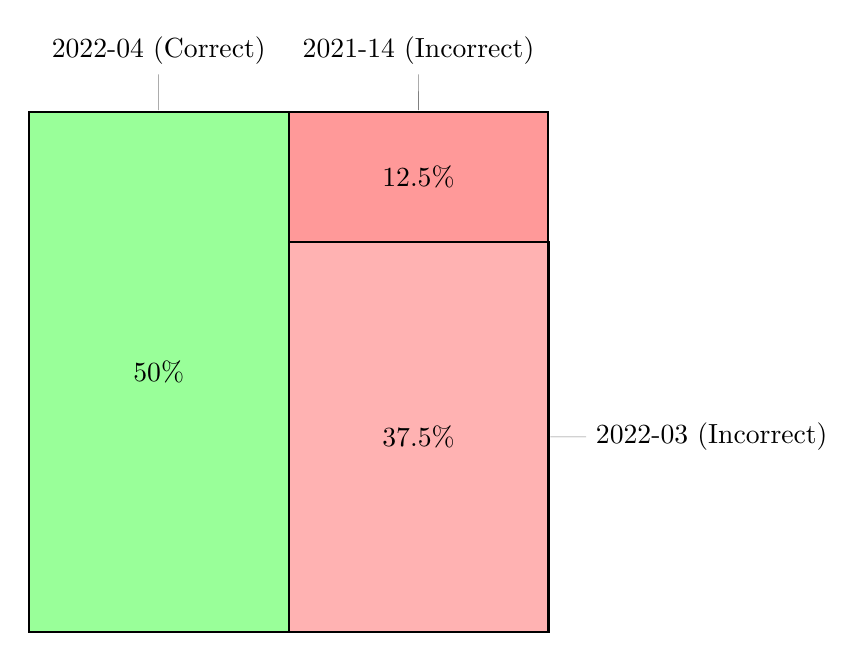
\begin{tikzpicture}[scale=1.1]
        \pie[square, text=pin, color={green!40, red!30, red!40}, rotate=180]{50/2022-04 (Correct), 37.5/2022-03 (Incorrect), 12.5/2021-14 (Incorrect)}
    \end{tikzpicture}
    \captionof{figure}{Question 5 Results}
\end{minipage}
\hfill
\begin{minipage}[t]{0.35\textwidth}
    \centering
    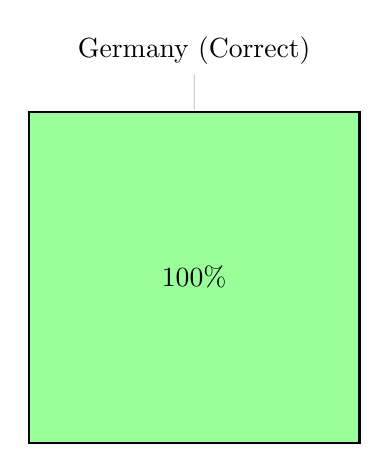
\begin{tikzpicture}[scale=0.7]
        \pie[square, text=pin, color={green!40, red!30, red!40}]{100/Germany (Correct)}
    \end{tikzpicture}
    \captionof{figure}{Question 6 Results}
\end{minipage}

\newpage
Overall, I am happy with the results of the user testing. My worst answered question was question 5, where only 50\% of users got the question correct. This was somewhat expected as the question required the user to use the program in a way that was not initially intended. The question was asking the user to find the peak case count of a country, which is not a feature of the program. The users were able to find the data, but they were not able to find the peak case count. This is something I will be looking to improve in the future.

\section{User Feedback}
The users were overall happy with the application. They liked the design and the way the data was presented. The users also liked the interactivity of the map and how they could zoom in on countries.\\

However, I received many suggestions for improvement, some of which I will be implementing. The main suggestions were:
\begin{itemize}
    \item The zoom button was not clear and the users did not know how to activate it.
    \begin{itemize}
        \item The button was hard to identify and it was not clear what it did. I will be changing the button to a more recognisable icon and adding a tooltip to explain what it does.
        \item The current behaviour of the button shows a globe icon when the map is not in zoom mode, and a zoom icon when the map is in zoom mode. This is not clear and I will be inverting the icons.
    \end{itemize}
    \item The search bar was not clear and the users did not know how to use it.
    \begin{itemize}
        \item The behaviour of the search bar and the comparison search bar were slightly different and one required the enter key to be pressed. I will be changing the search bar to behave the same as the comparison search bar.
        \item The search icon was not a button like the users expected. I will be changing the search icon to a button and adding a tooltip to explain what it does.
    \end{itemize}
    \item The users wanted the graphs to be viewable on a separate, larger window.
    \begin{itemize}
        \item This is a good idea, however the code base is not set up for this. I will be looking into this in the future, but it is not a priority at the moment.
    \end{itemize}
    \item Functionality to right click a country to add country to comparison graph.
    \begin{itemize}
        \item I will not be implementing this feature as it does not follow good UX design. Adding a country implicitly is a better solution.
    \end{itemize}
    \item Searching for a country did not highlight the country on the map.
    \begin{itemize}
        \item This is actually an intended feature, and was a bug in the code. I added a fix to highlight the country when it is selected.
    \end{itemize}
\end{itemize}

\newpage

\chapter{Conclusion}
In undertaking this project, I have met the objectives set. I have learned how to use multiple new technologies and how to use them together. I have also learned how to use Docker to deploy my application and how to use the fetch API to fetch data.\\

The web application was well received by the testers and they were able to use it to extract information from the data. The application is interactive and allows the user to zoom in on countries. The application is also able to display the data in a meaningful way.

\begin{center}
    \begin{figure}[h]
        \centering
        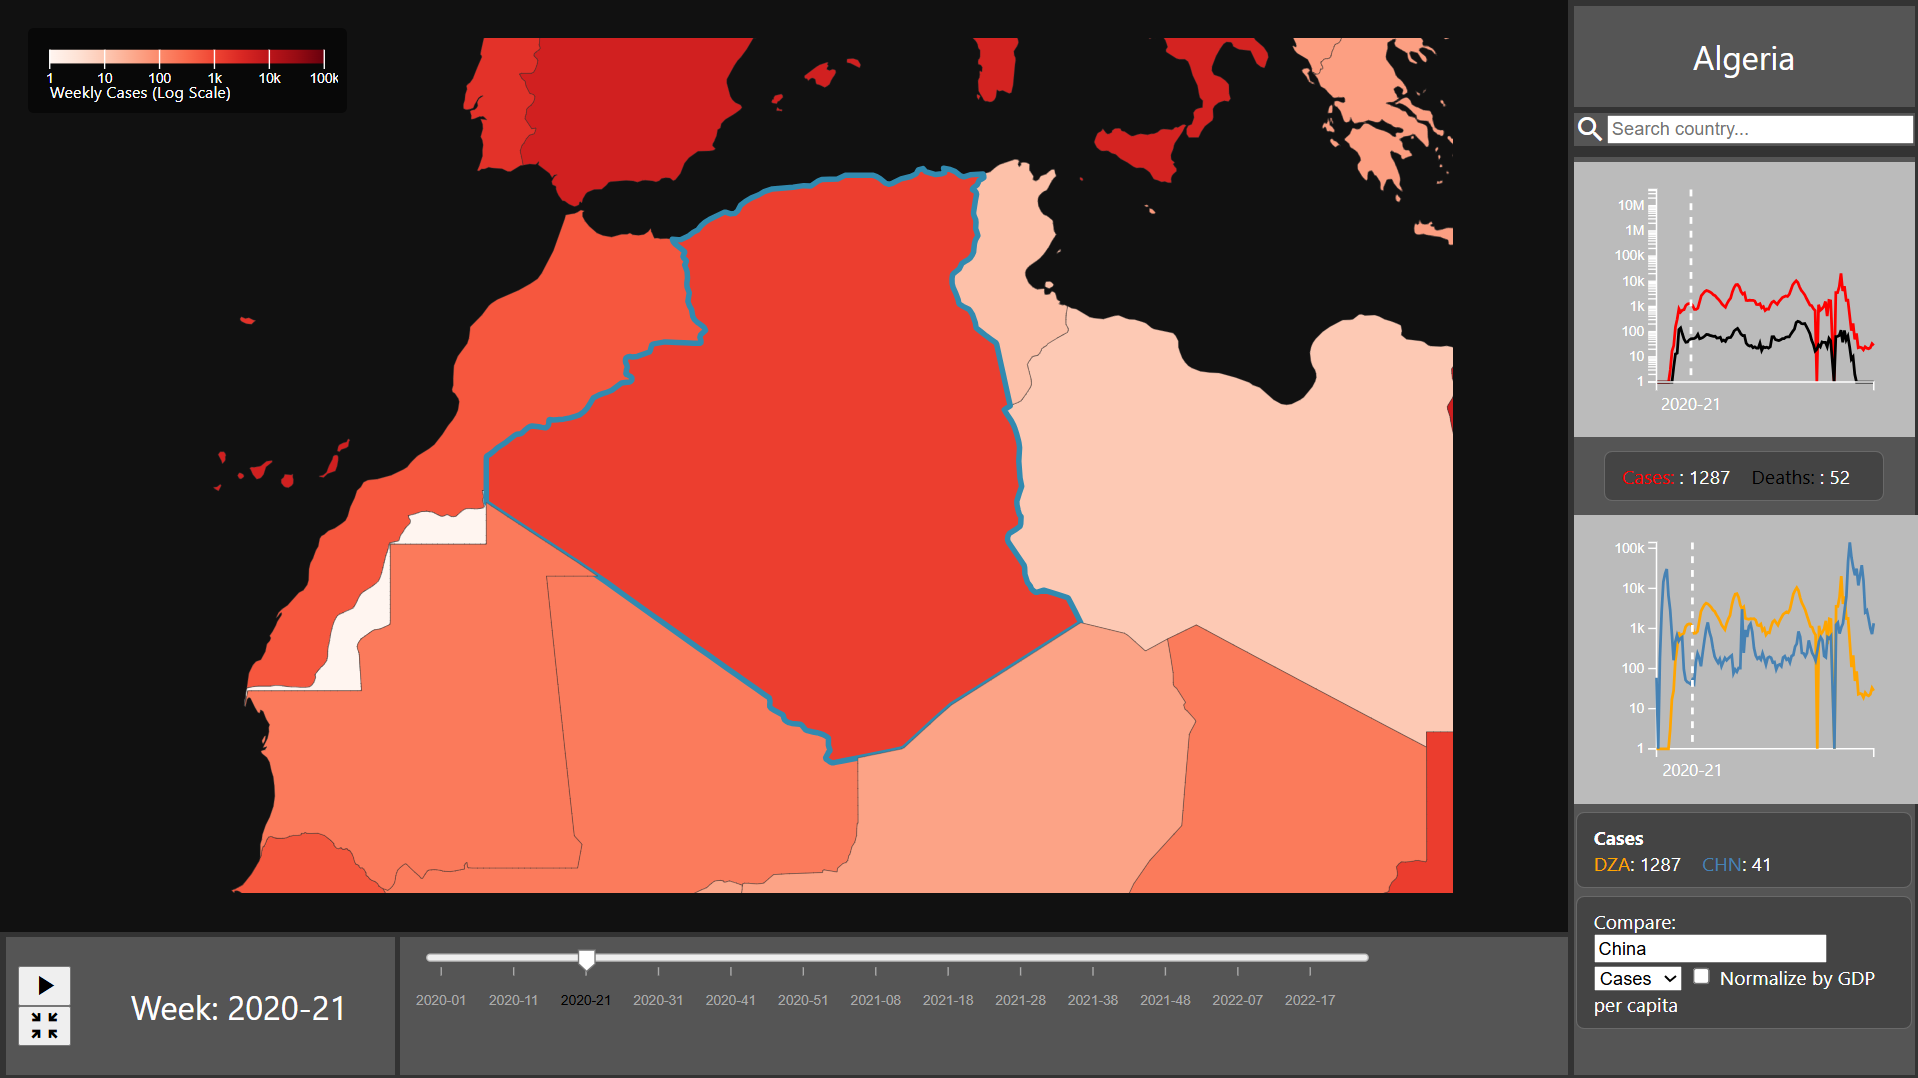
\includegraphics[width=0.95\textwidth]{Images/dashboard.png}
        \caption{Application Screenshot}
        \label{fig:dashboard-conc}
    \end{figure}
\end{center}
I have created a tool which can be used to visualise and analyse an arbitrary pandemic dataset. The tool is able to display the data in a meaningful way and can be used to find trends in the data. It can also be used to compare countries and find out which countries are doing better or worse than others.\\
\newpage

\chapter{Glossary}
\begin{itemize}
    \item \textbf{Choropleth Map} - A map in which areas are shaded or patterned in proportion to the value of a variable being represented.
    \item \textbf{D3.js} - A JavaScript library, Data-Driven-Documents, used for producing dynamic, interactive data visualisations in web browsers.
    \item \textbf{JSON} - JavaScript Object Notation, a lightweight data interchange format that is easy for humans to read and write and easy for machines to parse and generate.
    \item \textbf{GeoJSON} - A format for encoding a variety of geographic data structures using JSON.
    \item \textbf{Node.js} - An open-source, cross-platform, back-end JavaScript runtime environment that executes JavaScript code outside a web browser.
    \item \textbf{SIR Model} - A simple compartmental model used in epidemiology to simulate the spread of infectious diseases.
    \item \textbf{Epidemic} - A sudden increase in the number of cases of a disease above what is normally expected in a population in a given area.
    \item \textbf{Pandemic} - An epidemic that has spread across a large region, for instance multiple continents or worldwide.
    \item \textbf{Docker} - A platfirm for developing, shipping, and running applications in containers.
    \item \textbf{ISO-3166-1} - The International Organization for Standardization (ISO) standard for country codes.
    \item \textbf{SVG} - Scalable Vector Graphics, an XML-based vector image format for two-dimensional graphics with support for interactivity and animation.
\end{itemize}
\newpage

\bibliographystyle{plain} % We choose the "plain" reference style
\bibliography{refs} % Entries are in the refs.bib file
\newpage

\chapter{Appendix}
\section{restructure-json.py}
\begin{lstlisting}[language=Python]
    import json
    from collections import defaultdict
    
    #####################################################
    #ENTER UNCLEANED JSON FILE, e.g. "data.json"
    oldJSONFile = "data.json"
    #####################################################
    
    # Load JSON data from file
    with open(oldJSONFile, "r", encoding="utf-8") as infile:
        json_data = json.load(infile)
    
    # Data structure to hold per-country data
    countries = defaultdict(lambda: {
        "properties": {},
        "data": defaultdict(lambda: {
            "cases": 0,
            "deaths": 0,
            "cumulative_cases": 0,
            "cumulative_deaths": 0,
            "rate_14_day_cases": 0.0,
            "rate_14_day_deaths": 0.0
        })
    })
    
    # Initialize global totals
    world_totals = defaultdict(lambda: {
        "cases": 0,
        "deaths": 0,
        "cumulative_cases": 0,
        "cumulative_deaths": 0
    })
    world_population = 0  # We will sum all populations
    
    for entry in json_data:
        country = entry.get("country", "Unknown")
        country_code = entry.get("country_code", "N/A")
        
        # Populate country properties once
        if not countries[country_code]["properties"]:
            countries[country_code]["properties"] = {
                "country": country,
                "country_code": country_code,
                "continent": entry.get("continent", "Unknown"),
                "population": entry.get("population", 0),
                "source": entry.get("source", "Unknown")
            }
            world_population += entry.get("population", 0)  # Sum global population
    
        # Use the original year_week format (YYYY-WW)
        year_week = entry.get("year_week", "Unknown")
    
        # Extract indicator and values
        indicator = entry.get("indicator", "").lower()
        weekly_count = entry.get("weekly_count", 0)
        cumulative_count = entry.get("cumulative_count", 0)
        rate_14_day = entry.get("rate_14_day", 0.0)
    
        ################################################################
        # AMEND THIS AREA TO FIX TO YOUR OWN JSON FILE
        
        # Store values based on indicator type
        if indicator == "cases":
            countries[country_code]["data"][year_week]["cases"] = weekly_count
            countries[country_code]["data"][year_week]["cumulative_cases"] = cumulative_count
            countries[country_code]["data"][year_week]["rate_14_day_cases"] = rate_14_day
    
            # Add to world totals
            world_totals[year_week]["cases"] += weekly_count
            world_totals[year_week]["cumulative_cases"] += cumulative_count
    
        elif indicator == "deaths":
            countries[country_code]["data"][year_week]["deaths"] = weekly_count
            countries[country_code]["data"][year_week]["cumulative_deaths"] = cumulative_count
            countries[country_code]["data"][year_week]["rate_14_day_deaths"] = rate_14_day
    
            # Add to world totals
            world_totals[year_week]["deaths"] += weekly_count
            world_totals[year_week]["cumulative_deaths"] += cumulative_count
    
    
        ################################################################
            
    # Add global totals as a "World" entry
    countries["WORLD"] = {
        "properties": {
            "country": "World",
            "country_code": "WORLD",
            "continent": "Earth",
            "population": world_population,
            "source": "Aggregated Data"
        },
        "data": world_totals
    }
    
    # Convert defaultdict to normal dict for JSON output
    final_result = {country_code: {"properties": data["properties"], "data": dict(data["data"])} 
                    for country_code, data in countries.items()}
    
    # Write output to a new JSON file
    with open("pandemicData.json", "w", encoding="utf-8") as outfile:
        json.dump(final_result, outfile, indent=4)
    
    print("Data successfully transformed and saved to 'pandemicData.json'")
\end{lstlisting}
\newpage
\section{Gantt Chart}
    \begin{center}
        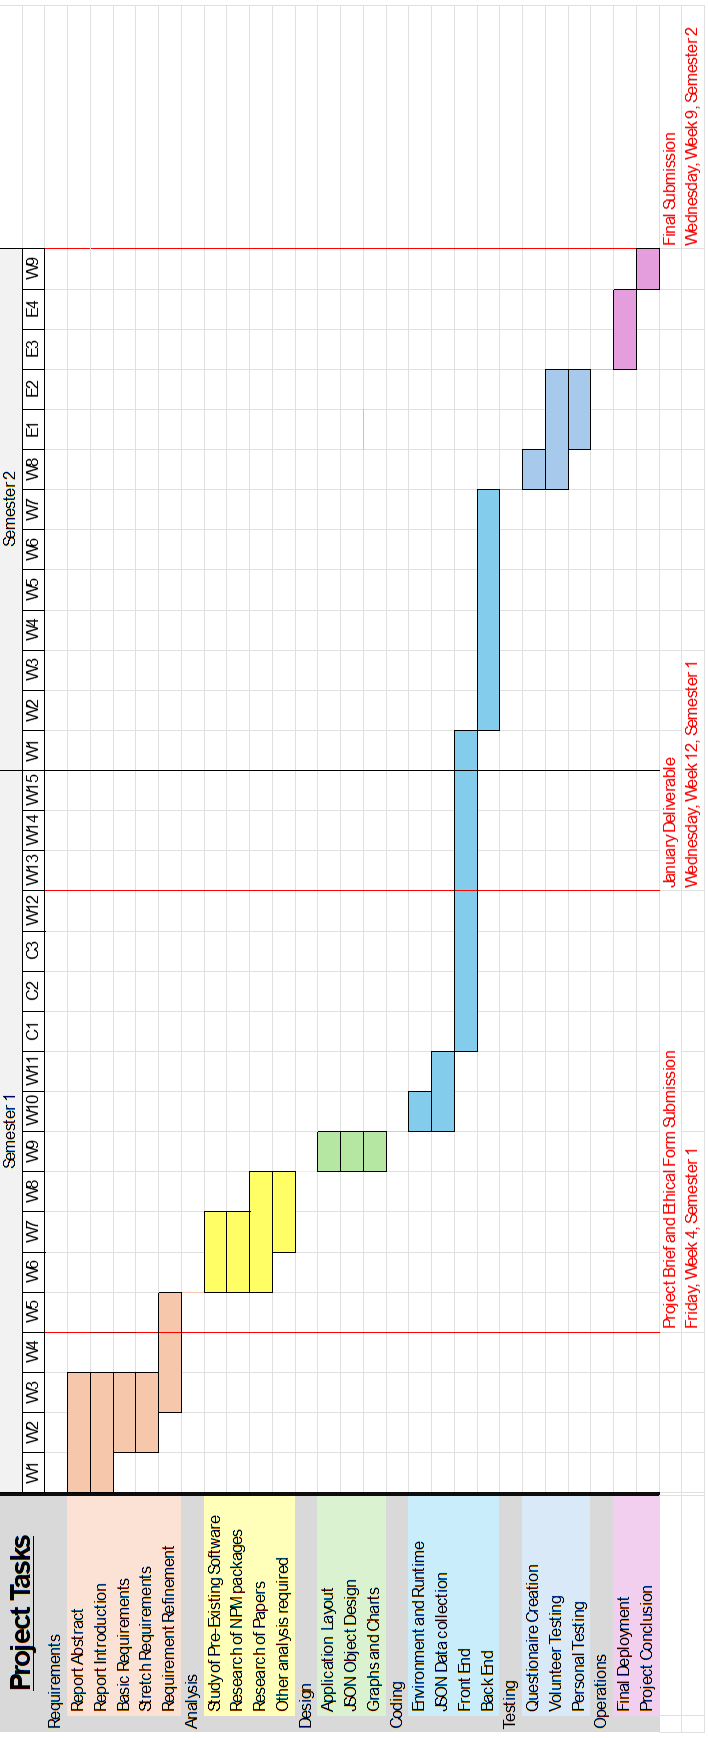
\includegraphics[height=0.95\textheight]{gantt_chart}
    \end{center}
\end{document}